%%=============================================================================
%% Methodologie
%%=============================================================================

\chapter{\IfLanguageName{dutch}{Methodologie}{Methodology}}
\label{ch:methodologie}
In dit deel van de thesis wordt eerst overlopen aan welke voorwaarden container virtualisatie software zou moeten voldoen om te kunnen dienen als leermiddel. Vervolgens worden deze voorwaarden afgetoetst aan de gevonden software om zo een aantal software combinaties bruikbaar voor testomgevingen te definiëren. Hierna worden het verloop en de eerste bevindingen van deze tests behandeld om af te sluiten met een algemeen resultaat.

%% Hoe ben je te werk gegaan? Verdeel je onderzoek in grote fasen, en
%% licht in elke fase toe welke stappen je gevolgd hebt. Verantwoord waarom je
%% op deze manier te werk gegaan bent. Je moet kunnen aantonen dat je de best
%% mogelijke manier toegepast hebt om een antwoord te vinden op de
%% onderzoeksvraag.

\section{Selectie criteria software}
Om container virtualisatie software te vinden die toepasbaar is om gebruikt te worden als lesmateriaal moet er aan bepaalde vereisten voldaan worden:

\begin{itemize}
    \item Kosteloos zijn: als er kosten zijn mogen deze de leerervaring niet ten nadele komen.
    \item Uitvoerbaar op de computers van de studenten. De gekozen software mag ook bij de verschillen in besturingssystemen van de studentencomputers niet te veel verschillen in werking.
    \item De software moet op zichzelf of in combinatie met andere software de volledige levenscyclus van containers kunnen tonen en niet te restrictief in gebruik zijn.
    \item Niet te complex zijn om te gebruiken.
    \item Geen verwaarloosde software zijn (nog voldoende ondersteuning beschikbaar).
\end{itemize}
    
\subsection{Algemene toepassingsvoorwaarden op gevonden software}
Door een klassieke VM te gebruiken om in te werken kunnen de problemen met de uitvoerbaarheid op het Host besturingssysteem van een studentenlaptop vermeden worden en zal de ingebruikname ook binnen de VM voor alle studenten hetzelfde zijn. Dit heeft ook het voordeel dat het besturingssysteem van de VM een Linux distributie kan zijn, een voorwaarde die moet vervuld zijn om veel van de besproken container virtualisatie software te kunnen draaien. De rest van deze sectie zal specifieker de gevonden technologieën overlopen.

Met uitzondering van technologieën die op Cloud berusten, de repositories of volledige Cloud services, zijn alle de gevonden technologieën gratis te gebruiken. Ook is er door het OCI een zekere mate van modulariteit tussen de technologieën. De gekozen software mag dan zelf niet de volledige levenscyclus kunnen ondersteunen, er zal altijd wel een zekere vorm van integratie zijn met software dit dat wel kan.

\subsection{Engines en runtimes}
Qua geschiktheid om als runtime en engine gebruikt te worden komen de Docker Engine en Podman als bestenaar voren. Docker dankzij zijn populariteit en veelzijdigheid. Bovendien is er ook veel onlinehulp te vinden voor het gebruik van Docker. Podman’s vriendelijkheid als leermiddel is dan weer te verklaren doordat het zich opstelt als een duidelijk alternatief voor Docker op Linux distributies en ook veel nabootst van Docker. De directe hulp en uitleg om met Podman te werken is echter minder uitgebreid. Verder zou Containerd ook nog een alternatief kunnen zijn, maar dan nipt wat betreft de complexiteit van het gebruik, zeker in vergelijking met Podman en Docker. Tabel \ref{tab:Engines} toont van deze en de andere grotere gevonden engines, runtimes of containers hun restricties en complexiteiten. 

Het zelf werken met Linux containers is te complex om een goede introductie tot container virtualisatie te zijn. Windows containers zijn enkel mogelijk op bepaalde distributies van Windows en berusten verder op de Docker engine voor de uitvoering, hierdoor biedt de extra stap om met deze containers te werken ten opzichte van Docker geen meerwaarde als inleiding. Doordat CRI-O gericht is op integratie met Kubernetes is het niet geschikt om containers te gebruiken zonder al meteen met orchestration te werken. Het unieke verkoopsargument van Kata containers, de mogelijkheid om ook VM’s als containers te draaien, is een stap in complexiteit die te ver gaat om een goede inleiding tot container virtualisatie te zijn. De rest van de gevonden runtimes zijn te beperkt qua gebruik of al te lang zonder ondersteuning om met zekerheid te kunnen zeggen dat ze relevant zullen blijven voor containers en verwante technologieën. 


\begin{center}
    \begin{table}
    \begin{tabular}{ m{3.5cm} || m{1cm} | m{3.3cm} | m{4.5cm} }
        Engine/container & Gratis & Besturingssysteem restricties & Bijkomende complexiteit t.o.v. Docker \\ 
        \hline
        Docker & ja & geen &  \\  
        \hline
        Containerd & ja & De meeste Linux distributies & Werkt voor sturing met Go programma’s \\
        \hline 
        Linuxcontainers & ja & Linux & Zelf configureren via het besturingssysteem \\
        \hline
        Cri-o & ja & De meeste Linux distributies & Enkel voor werking met Kubernetes \\
        \hline
        Podman & ja & De meeste Linux distributies & Veel overgenomen van Docker + Ingebouwde pods \\
        \hline
        Windows containers & ja & Windows, exlusief Home Edities & Werkt enkel met Docker/ Niet van toepassing \\
        \hline
        PouchContainer & ja & Ubuntu of CentOS & Slechte documentatie \\
        \hline
        Kata containers & ja & De meeste Linux distributies & Extra configuratie, nood aan Containerd of Cri-o voor uitvoering \\
    \end{tabular}
    \caption[Overzicht Runtimes en containers]{Een overzicht van gevonden runtimes of containers met hun restricties en bijkomende complexiteit.}
    \label{tab:Engines}
    \end{table}
\end{center}

\subsection{Orchestration}
Docker Compose is een uitbreiding van de Docker engine en is daarmee ook gratis en heeft dezelfde vereisten als Docker. Het wordt zelfs standaard geïnstalleerd met de Docker desktop applicatie maar het is geen volledige orchestration software. Kubernetes en Nomad zijn verder nog twee softwarepakketten die goed zouden kunnen zijn om met te leren. Kubernetes is de meest gebruikte orchestration software en is daarmee zoals Docker voorzien van veel online hulp. Het is open source en kan met veel van de runtimes werken. Voor het leren werken met Kubernetes is er ook Minikube die je lokaal in staat stelt met Kubernetes te werken. Nomad is orchestration software die lijkt op Kubernetes maar toch zichzelf wilt onderscheiden van Kubernetes door meer dan alleen containers te kunnen beheren. Tabel \ref{tab:Ochestration} toont voor de orchestration software een overzicht.

\begin{center}
    \begin{table}
        \begin{tabular}{ m{3cm} || m{1.5cm} | m{3.3cm} | m{4.5cm} }
            Software & Gratis & Besturingssysteem restricties & Bijkomende complexiteit t.o.v. Docker \\ 
            \hline
            Docker Compose & ja & geen &  \\  
            \hline
            Docker Swarm & ja & geen & \\
            \hline 
            Kubernetes & ja & geen & Minikube als middleware voor lokale uitvoering \\
            \hline
            OpenShift & 30-day trail & Red Hat Besturingsystemen & Zelf datacenter opzetten of Cloud gebruiken \\
            \hline
            Nomad & ja & geen & Eigen configuratie taal \\
            \hline
            Apache Mesos & ja & geen & Met binary of zelf lokaal builden.  \\
            \hline 
            DC/OS & ja & DC/OS & Zelf datacenter opzetten \\
        \end{tabular}
        \caption[Overzicht orchestration]{Een overzicht van gevonden orchestration software met hun restricties en toegevoegde complexiteit.}
        \label{tab:Ochestration}
    \end{table}
\end{center}

Het feit dat DC/OS orchestration gebonden is aan een specifiek besturingssysteem of dat men een volledig datacenter moet opzetten voor Apache Mesos of OpenShift maakt deze software te complex om te kunnen dienen als een introductie tot orchestration bij container virtualisatie. En tenslotte is er nog de Docker Swarm die zelf aan populariteit verliest ten opzichte van Kubernetes als software voor orchestration en waar ook vaak wordt voorgesteld om het te vervangen door Kubernetes.


\subsection{Image repositories}
Doordat het OCI met hun container image er in geslaagd is om container images te standaardiseren zijn repositories vrij met elkaar te wisselen. De Docker Hub en de GitHub Container Registry zijn de meest geschikte om door een student als image repository te gebruiken. Docker Hub doordat het bijna overal als standaard gebruikt wordt en de GitHub Container Registry omdat een student wellicht al een GitHub account zal hebben. Ook de kostenstructuur van de twee is te vergelijken met gratis publieke images en betaling vanaf een bepaalde drempel voor private images. Tijden het schrijven van deze thesis was de GitHub Container Registry wel nog in een bètafase waardoor het volledig gebruik gratis is. Een overzicht van deze twee en de GitLab Container Registry staat in tabel \ref{tab:repositories}.

\begin{center}
    \begin{table}
        \begin{tabular}{ m{3.5cm} || m{2cm} | m{3.3cm} | m{4.5cm} }
            Repository & Gratis Account & Limiet gratis privé images & Overdracht limiet \\ 
            \hline
            Docker Hub & ja & 1 image & 100 per 6 uur anoniem en 200 per 6 uur ingelogd
             \\  
            \hline
            GitHub Container Registry & ja & 500 mb* & Niet gespecifieerd \\
            \hline 
            GitLab Container Registry & 30-day trail & Niet gespecifieerd & Niet gespecifieerd \\
            \multicolumn{4}{c}{ } \\
            \multicolumn{4}{l}{*In bèta waren geen limieten van toepassing, het zal de GitHub Packages limieten delen.} \\
        \end{tabular}
        \caption[Overzicht image repositories]{Een overzicht van gevonden image repositories met hun limieten voor gratis accounts.}
        \label{tab:repositories}
    \end{table}
\end{center}

\subsection{Cloud hosting en services}
Cloud hosting services kunnen een optie zijn maar afhankelijk van de host kan het dat een gratis proefperiode niet toegang geeft tot alle tools die nodig zijn of dat het moeilijk is om gratis krediet te krijgen. Zo verleent Amazon geen gratis krediet of vraagt Google om een kredietkaart in te geven om recht op gratis krediet te krijgen. Verder zal het maken van een nieuwe image eerst lokaal moeten gebeuren waarvoor een lokale runtime nodig is. Hierdoor kan er even goed in eerste instantie lokaal verder gewerkt worden.

\section{Software Tests}
Wegens de modulariteit gecreëerd door het OCI zullen we in de test eerst de runtimes uitproberen, om daarna te kijken naar de mogelijkheden van de runtimes om te werken met orchestration software.

\subsection{Engines en runtimes}
Voor deze testen is het vooral van belang dat containers en hun images kunnen gemaakt gedraaid en gestopt worden door middel van de runtime en engine. Ook moet het mogelijk zijn om data te persisteren naar een volume.

\paragraph{Docker Desktop}
De Docker desktop is een applicatie voor Windows en Mac die de Docker engine combineert met Docker Compose, lokale Kubernetes, een dashboard en een eenvoudige verbinding met de Docker Hub. Wegens de volledigheid van deze bundel werd dit als eerste uitgeprobeerd. Doordat de desktop applicatie niet voor Linux bestaat is deze bundel echter niet volledig toepasbaar voor alle studenten. Een Linux gebruiker zou de delen apart moeten installeren. Dit is ook de software die direct op een laptop zal worden uitgevoerd en niet in een VM. Deze combinatie zal gebruikt worden als een baseline voor vergelijkingen. 

\paragraph{Fedora Podman}
Een eerste VM waarin het meest beloftevolle alternatief Podman wordt getest is een Fedora workstation instantie. Deels omdat Fedora al gebruikt wordt tijdens het vak besturingssystemen en omdat het ook standaard met een Firefox webbrowser komt wat het gemakkelijk maakt om te testen of een webservice-gebaseerde container correct draait.

\paragraph{Ubuntu Podman}
Om Podman ook uit te proberen op een ander besturingssysteem dan Fedora werd ook eens geprobeerd of het lukt om Podman te installeren op een Ubuntu distributie.

\subsection{Orchestration}
Voor orchestration moet het mogelijk zijn om een job of taak op basis van containers aan te maken, aan te passen en te stoppen. En ook om iets complexer dan een enkele container service te draaien.

\paragraph{Kubernetes gebundeld met Docker desktop}
De Docker desktop applicatie komt met de mogelijkheid om een lokale Kubernetes instantie te starten. Het lijkt dus interessant om deze combinatie ook eens te testen.

\paragraph{Podman met Minikube voor Kubernetes}
Om te testen of het ook mogelijk is om met Podman als runtime te werken voor Kubernetes werd er ook geprobeerd om een Minikube instantie, werkende met Podman, op te zetten en te gebruiken.

\paragraph{Docker engine en Nomad}
In tegenstelling tot Kubernetes en Minikube die meer vrijheid hebben voor de achterliggende runtime biedt Nomad op dit moment enkel ondersteuning voor de Docker engine om mee te werken voor het draaien van een containers. Als we Nomad wensen uit te proberen moet er dus met een Docker engine gewerkt worden.

\section{Verloop en resultaten softwaretests}
In dit deel worden per opgestelde software test de nodige voorbereiding, het effectieve gebruik en ondervindingen overlopen. 

\subsection{Docker Desktop} \label{DockerDesktop}
Het eerste dat uitgeprobeerd werd is de Docker desktop geïnstalleerd als applicatie op een Windows Home editie laptop met 8 GB ram geheugen.

\paragraph{Installatie en set-up}
Om te kunnen werken met Docker desktop direct geïnstalleerd op een Windows systeem moet er eerst het Windows Subsysteem voor Linux (WSL) ingeschakeld worden. Docker verwijst hiervoor naar de help pagina’s van Microsoft. Hierbij werden de manuele instructies van Microsoft \footnote{\url{https://docs.microsoft.com/en-us/windows/wsl/install-win10}} gevolgd om tot en met het opzetten van WSL2 als default uit te voeren. Het enige dat hier wat specifieke aandacht vereist ten opzichte van de beschreven stappen is het controleren of de Windows versie geschikt is voor WSL.

Hierna werd de installer van de Docker desktop uitgevoerd. Deze installer heeft een optie om WSL voor de gebruiker voor te bereiden, maar omdat dit reeds gedaan was is konden we niet testen of deze optie het volledig ennablen van WSL doet of enkel verantwoordelijk is voor het instellen van een Linux distributie in WSL waarmee de containers zullen kunnen worden uitgevoerd.


\paragraph{Ingebruikname}
Bij het eerste keer opstarten van de desktop applicatie wordt een korte tutorial getoond die enkel het pullen, builden en uitvoeren van een eenvoudige container behandelt.Dit is deels een zeer korte introductie en een test om te zien of de installatie wel gelukt is. Het opstarten van de desktop applicatie is ook de trigger om de backend die alles effectief draait ook te starten.

\begin{lstlisting}[caption=inhoud van de Dockerfile,label=lst:Dockerfile]
FROM node:12-alpine
RUN apk add --no-cache python g++ make
WORKDIR /app
COPY package.json yarn.lock ./
RUN yarn install --production
COPY . .
CMD ["node", "src/index.js"]
\end{lstlisting}

Vervolgens werd een uitgebreide tutorial van Docker gevolgd\footnote{\url{https://docs.docker.com/get-started/02_our_app/}}. Dit begon met het kopiëren van een kleine todo-list webapplicatie gemaakt met node.js, , gehost op GitHub\footnote{\url{https://github.com/docker/getting-started/tree/master/app}}. Voor het builden van de container wordt een dockerfile gebruikt, te zien in listing \ref{lst:Dockerfile}. Door dit op te slaan in de root van de webapplicatie kan volgend commando uitgevoerd worden in deze map voor het builden van de container.
\begin{verbatim}
docker build -t getting-started .
\end{verbatim}
Met dit commando wordt op basis van de dockerfile in de lokale map een image gemaakt en krijgt deze de tag “getting started”. Via de desktop applicatie, afgebeeld in figuur \ref{fig:Dockerdesktop}, of het commando `docker image ls' of `docker images` wordt een lijst van lokale images getoond waaronder de aangemaakte “getting started” image.
\begin{figure}[h]
    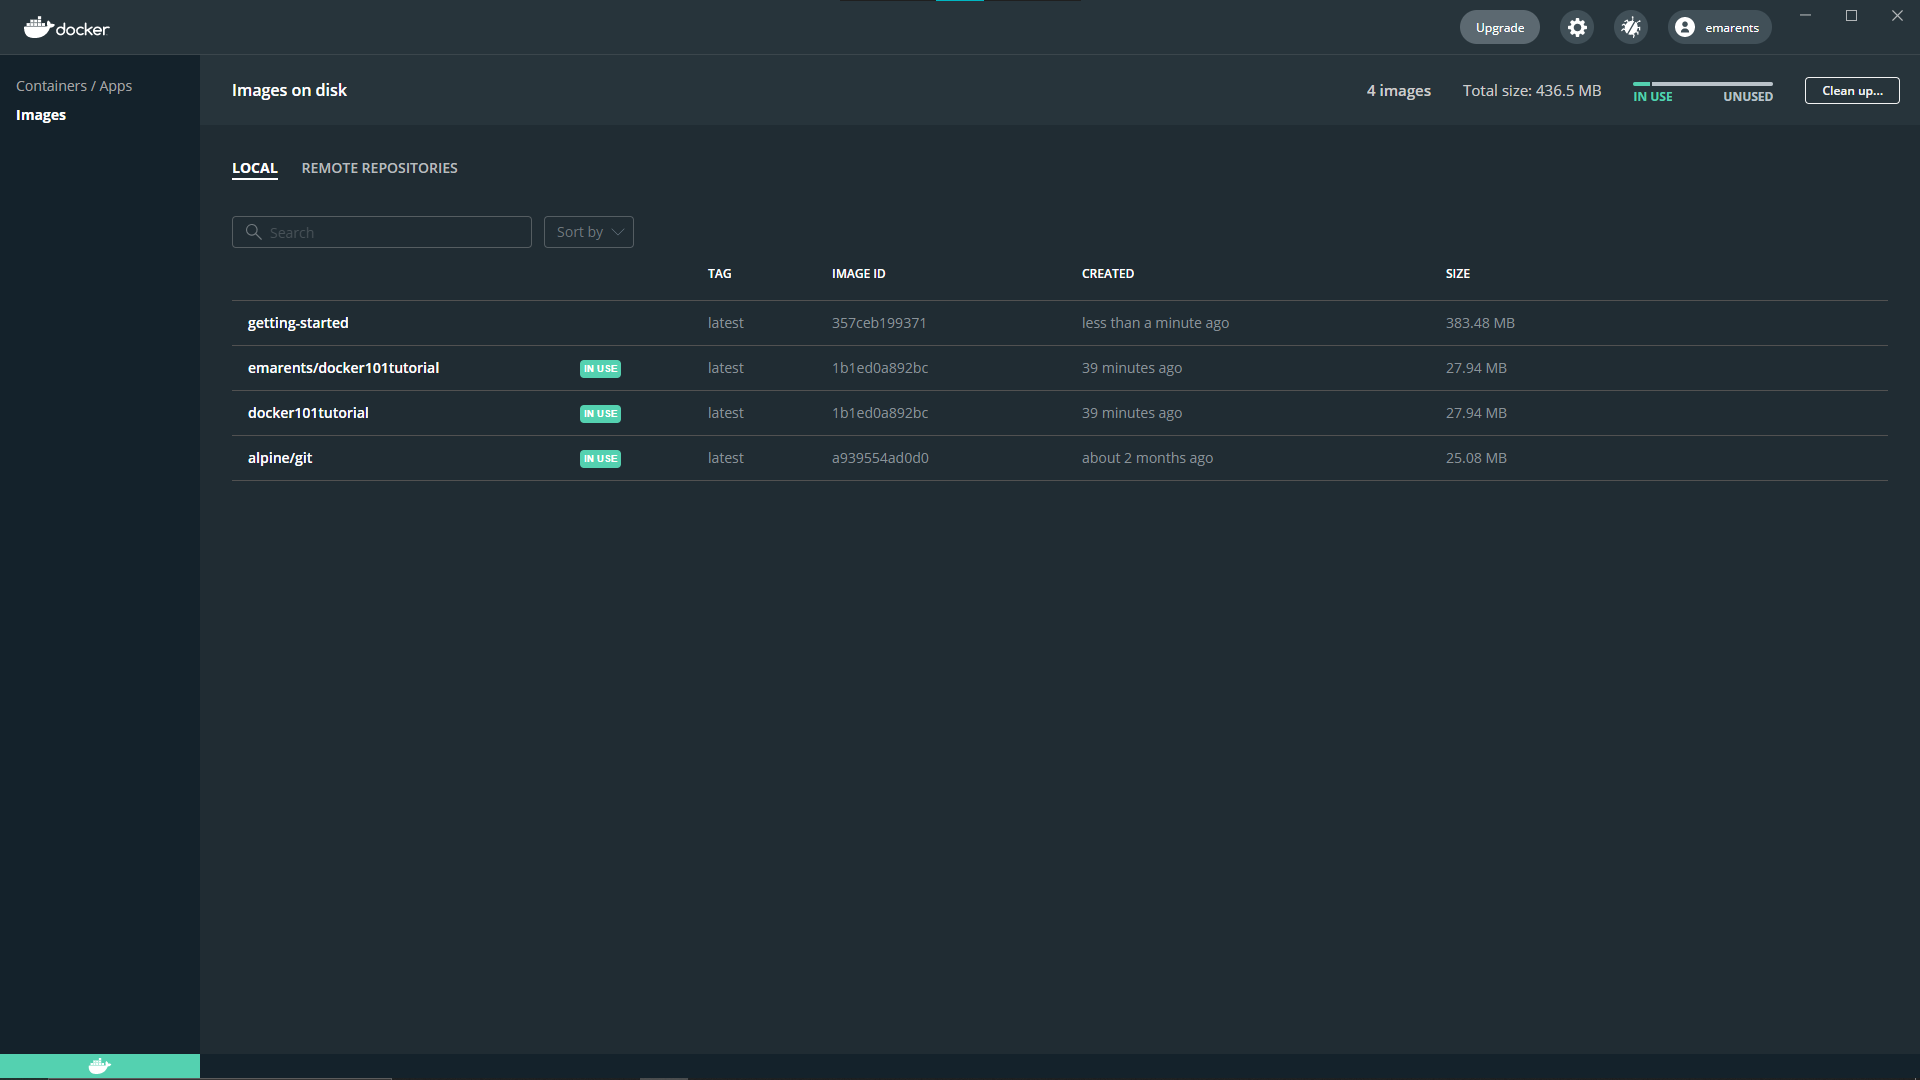
\includegraphics[width=\linewidth]{img/dockerImg.png}
    \caption[De Docker desktop applicatie]{De Docker desktop applicatie, dit deel toont alle lokaal bewaarde images}
    \label{fig:Dockerdesktop}
    \centering
\end{figure}
\begin{verbatim}
docker run -dp 3000:3000 getting-started
\end{verbatim}
Met dit commando wordt deze aangemaakte container uitgevoerd. ‘-p’ 3000:3000 stelt de port in zodat de webapplicatie via localhost:3000 bereikt kan worden. ‘-d’ voert de container detached uit waardoor de huidige actieve CLI niet vast wordt gehangen aan de opgestarte container.

Vervolgens werd in de bronbestanden de todo applicatie de placeholder tekst van de applicatie veranderd. Met deze aanpassing moet de image opnieuw worden gebuild. Vooraleer de nieuwe container met hetzelfde commando kan worden gestart moet de oude worden gestopt. Dit is mogelijk via de desktop applicatie of via CLI. Voor CLI moet ‘docker ps’ uitgevoerd worden om een lijst te krijgen van draaiende containers. In deze lijst van containers krijgt elke Container een ID. Met deze ID kan de container gestopt en verwijderd worden.
Het stoppen gebeurt met:
\begin{verbatim}
docker stop <container-id>
\end{verbatim}
En het verwijderen met:
\begin{verbatim}
docker rm <container-id>
\end{verbatim}
Door bij ‘docker rm’ de ‘-f’ vlag toe te voegen zal een container geforceerd gestopt worden vooraleer deze te verwijderen. . Ook is het mogelijk om de container ID te vervangen door de automatisch gegeneerde naam die Docker toekent aan een draaiende container.

Na het stoppen kan de nieuwe image met het run commando terug op dezelfde manier gestart worden.
\begin{verbatim}
docker run -dp 3000:3000 getting-started
\end{verbatim}
Vervolgens werd de container gepushed naar de Docker Hub. Hiervoor moet er eerst een account op de Docker Hub aangemaakt worden, en moet er voor dit account een nieuwe repository aangemaakt worden. Hiertoe werd dezelfde naam getting-started gebruikt en was de repository publiek. Om de lokale image te kunnen pushen moet de lokale Docker instantie ingelogd zijn. Dit gebeurt via volgend commando:
\begin{verbatim}
docker login -u USER-NAME
\end{verbatim}
Om juist de container te pushen naar je eigen repository moet de image een nieuwe tag krijgen die je gebruikersnaam en repository specificeert.
\begin{verbatim}
docker tag getting-started USER-NAME/getting-started
\end{verbatim}
Hierna kan de image naar de repository worden gepushed.
\begin{verbatim}
docker push USER-NAME/getting-started
\end{verbatim}
Op dit moment verliest de todo lijst in de applicatie nog alle gegevens wanneer de container word verwijderd dus moet er een volume gebruikt worden om de inhoud op te slaan. Hiervoor moet er eerst in Docker een volume worden aangemaakt:
\begin{verbatim}
docker volume create todo-db
\end{verbatim}
Vervolgens kan de applicatie weer opgestart worden met het run commando maar deze keer met een parameter voor de volume:
\begin{verbatim}
docker run -dp 3000:3000 -v todo-db:/etc/todos getting-started
\end{verbatim}
Als na het invullen van een item in de todo applicatie de container verwijderd word zal bij het opstarten van de container met hetzelfde commando de opgeslagen inhoud worden hergebruikt.

De gebruikte node.js applicatie werkt standaard met een SQLite database waarbij alles weggeschreven wordt naar een bestand. Dit bestand is wat er bewaard wordt in de volume om zo hergebruikt te worden. Deze applicatie kan echter ook met een externe SQL-databank werken. Dit kan dan ook opgezet worden via containers.

De eerste manier is door manueel zelf de containers te verbinden over het netwerk. Hiervoor moet er eerst een netwerk aangemaakt worden in Docker.
\begin{verbatim}
docker network create todo-app
\end{verbatim}
Vervolgens wordt een MySQL databank container gemaakt op dit netwerk. Hiervoor werd volgende commando gebruikt in Windows Powershell:
\begin{lstlisting}
docker run -d `
    --network todo-app --network-alias mysql `
    -v todo-mysql-data:/var/lib/mysql `
    -e MYSQL_ROOT_PASSWORD=secret `
    -e MYSQL_DATABASE=todos `
    mysql:5.7
\end{lstlisting}
Dit commando maakt een container van mysql:5.7 aan. De image die gebruikt wordt is de MySQL container versie 5.7 zoal deze te vinden is op de Docker Hub. De container wordt toegevoegd aan het netwerk en krijgt een alias. Het heeft ook een toewijzing voor het volume dat gebruikt moet worden. De parameters bij de -e vlaggen zijn environment variabelen die de MySQL instantie configureren. Door middel van volgend commando is het mogelijk om de CLI van de SQL-server te bereiken.

\begin{verbatim}
docker exec -it <mysql-container-id> mysql -u root -p
\end{verbatim}
Om te achterhalen hoe dat deze MySQL server terug te vinden is binnen het aangemaakte todo-app netwerk stelt Docker voor om binnen het netwerk een nicolaka/netshoot image te runnen en te gebruiken.
\begin{verbatim}
docker run -it --network todo-app nicolaka/netshoot
\end{verbatim}
Door in de interface van de netshoot ‘dig mysql' uit te voeren kan gekeken worden of het gebruikte netwerk alias bij het opstarten van de container effectief in het netwerk zit. Door volgend commando uit te voeren in de root folder van de todo-app zal een nieuwe container gestart worden. In deze nieuwe container gebaseerd op node:12-alpine wordt bij het starten de inhoud van de todo-app ingevoegd en worden de commando’s voor het starten van de app uitgevoerd.

\begin{lstlisting}
docker run -dp 3000:3000 `
    -w /app -v "$(pwd):/app" `
    --network todo-app `
    -e MYSQL_HOST=mysql `
    -e MYSQL_USER=root `
    -e MYSQL_PASSWORD=secret `
    -e MYSQL_DB=todos `
    node:12-alpine `
    sh -c "yarn install && yarn run dev"
\end{lstlisting}
Eens de container gestart is kunnen de log berichten van de containers opgevraagd worden of via hetzelfde commando als eerder de MySQL server aangesproken worden. Afbeelding \ref{fig:powershellsql} toont hoe in Windows Powershell de inhoud van de SQL databank opgehaald werd.
\begin{figure}[h]
    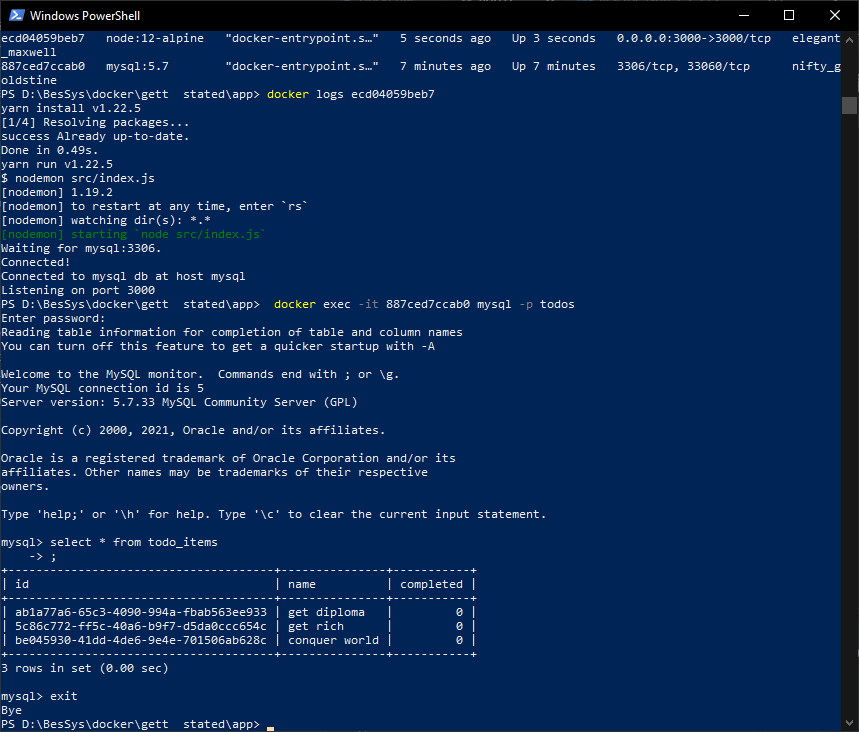
\includegraphics[width=\linewidth]{img/sqlquery.png}
    \caption[Het aanspreken van een SQL server binnen een container]{Met Docker is er in Powershell ingelogd op de SQL server die in een container staat om zo de inhoud op te halen.}
    \label{fig:powershellsql}
    \centering
\end{figure}

Omdat er veel stappen nodig zijn om op deze manier een applicatie te starten is er ook Docker Compose. Bij Docker Compose worden alle configuratiegegevens gedefinieerd in een YAML-configuratiebestand die vervolgens met Compose tot het builden en verbinden van de nodige containers leidt. De inhoud van het yml-bestand dat voor deze applicatie gebruikt werd staat in listing \ref{lst:Composefile}.

\begin{lstlisting}[caption=inhoud van de docker-compose.yml,label=lst:Composefile]
version: "3.7"

services:
    app:
        image: node:12-alpine
        command: sh -c "yarn install && yarn run dev"
        ports:
            - 3000:3000
        working_dir: /app
        volumes:
            - ./:/app
        environment:
            MYSQL_HOST: mysql
            MYSQL_USER: root
            MYSQL_PASSWORD: secret
            MYSQL_DB: todos

    mysql:
        image: mysql:5.7
        volumes:
            - todo-mysql-data:/var/lib/mysql
        environment: 
            MYSQL_ROOT_PASSWORD: secret
        MYSQL_DATABASE: todos

volumes:
todo-mysql-data:
\end{lstlisting}
Hierbij word voor de twee container services gedefinieerd welke base images elk moet gebruiken en de environment variabelen ingesteld. Ook hier wordt de node:12-alpine image lokaal gevuld met de te gebruiken inhoud. Voor het opstarten van de applicatie moet volgend commando worden uitgevoerd in de root map met het docker-compose.yml bestand.
\begin{verbatim}
docker-compose up -d
\end{verbatim}
Om het achteraf weer te stoppen kan op dezelfde plaats volgend commando uitgevoerd worden
\begin{verbatim}
docker-compose down 
\end{verbatim}
\paragraph{Ervaringen}
Het gebruik van Docker is eenvoudig en er is ook online veel hulpinformatie over te vinden bij eventuele problemen. De Docker Desktop heeft een grafische interface voor het beheren van draaiende containers en images, maar dit is ook allemaal mogelijk via de CLI. Met als belangrijke beperking dat bij het overnemen van commando’s deze commando’s soms over meerdere regels gespreid zijn en dat dus de commando prompt van Windows niet voldoende is en er overgeschakeld moet worden naar Powershell. De desktop interface maakt het wel gemakkelijk om te beheren of je lokale Docker instantie draait, waardoor het perfect mogelijk is om het geïnstalleerd te hebben staan en buiten gebruik niet door beïnvloed worden. Het starten en stoppen van Docker in een Linux omgeving is te controleren via het proces beheer van Linux zelf. De configuratie bestanden voor containers zijn geschreven in YAML en Visual Studio Code heeft zelf extensies om specifiek de Docker bestanden te ondersteunen.

\subsection{Fedora Podman}
Deze test werd uitgevoerd in een VM met 4 GB ram en 20 GB harde schijfruimte
\paragraph{Installatie en set-up}
Bij de verse installatie van een Fedora workstation versie 53 was Podman al inbegrepen en was er geen behoefte om deze apart te installeren.

\paragraph{Ingebruikname}
Voor het testen van het werken met Podman werden dezelfde stappen en begin bestanden gebruikt als in sectie \ref{DockerDesktop}. Dezelfde todo applicatie werd eerst lokaal gekopieerd en voorzien van een dockerfile/containerfile als in listing \ref{lst:Dockerfile}.

Voor het builden van de image gebruikt Podman het volgende commando, het uitvoeren ervan word getoond in figuur \ref{fig:podmanbuild}.
\begin{figure}[h]
    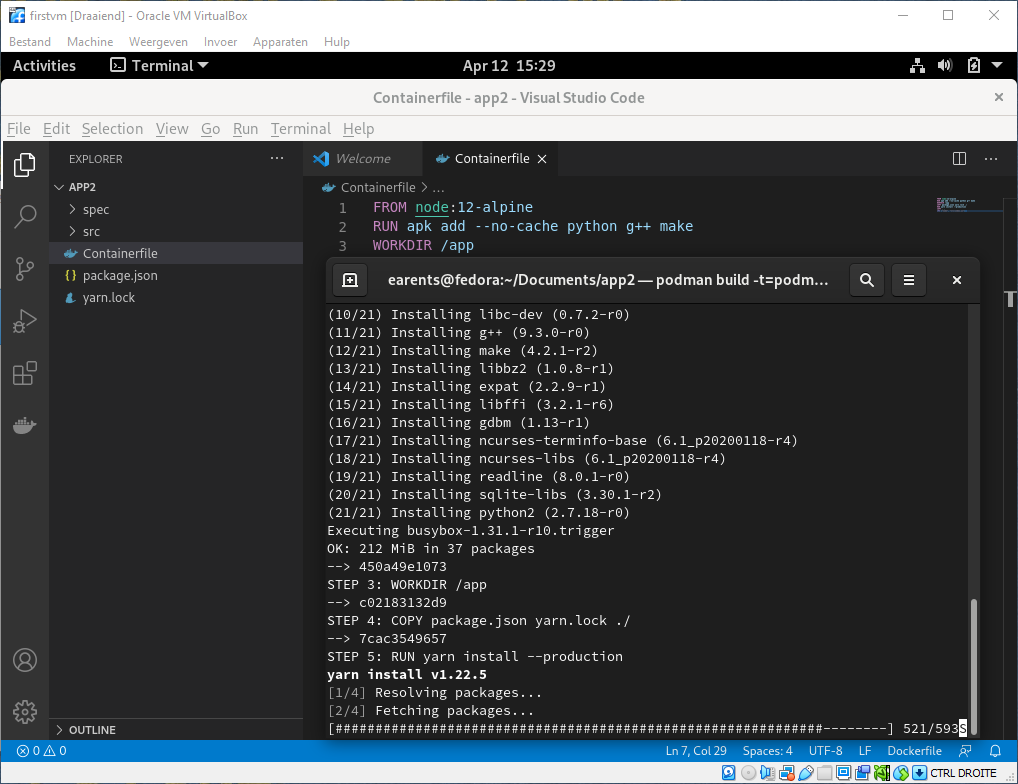
\includegraphics[width=\linewidth]{img/podmanbuild.png}
    \caption[Met podman een containerfile builden]{Hier maakt Podman met het inhoudelijk zelfde dockerfile/containerfile as Docker een image}
    \label{fig:podmanbuild}
    \centering
\end{figure}
\begin{verbatim}
Podman build -t getting-started .
\end{verbatim}
 
Op gelijkaardige wijze als bij Docker kan men de images opvragen met `podman images ls' of `podman images'. Ook het achterhalen van actieve containers gebeurt analoog met `podman ps'.

Vervolgens kan de container worden gestart met volgend comando, zoals ook te zien is in figuur \ref{fig:podmanrun}. 
\begin{figure}[h]
    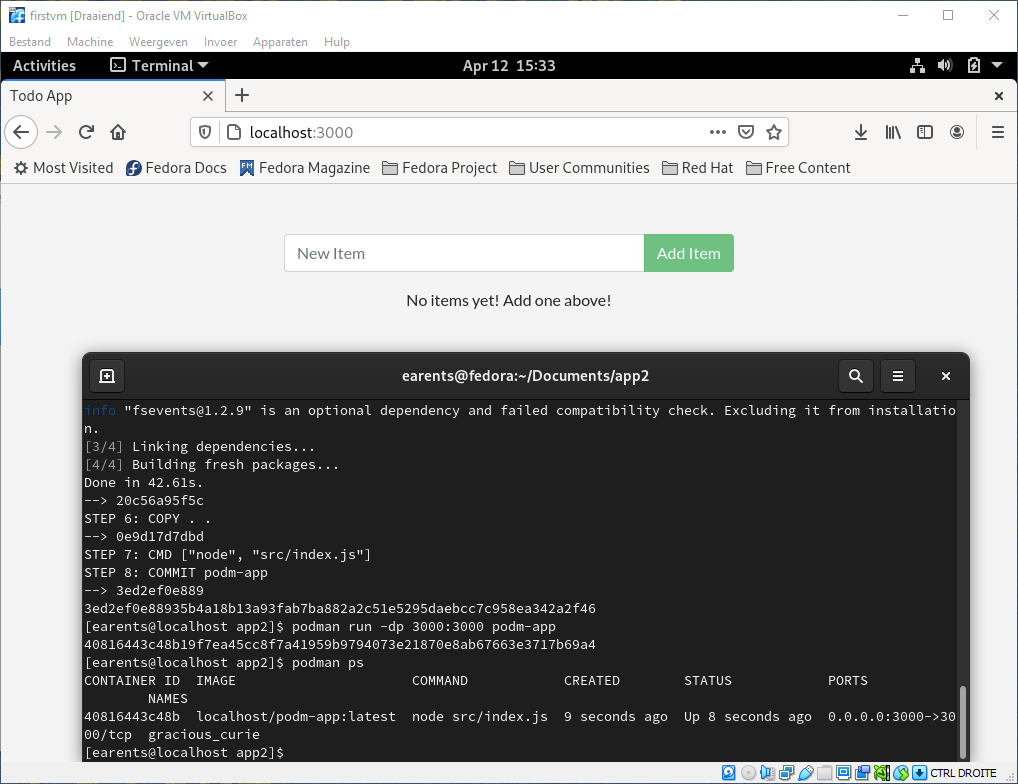
\includegraphics[width=\linewidth]{img/podmanrun.png}
    \caption[Podman die een web app uitvoert]{Hier is via command line de aangemaakte container gestart en wordt deze op de achtergrond getoond in een webbrowser.}
    \label{fig:podmanrun}
    \centering
\end{figure}
\begin{verbatim}
podman run -dp 3000:3000 getting-started
\end{verbatim}
Het stoppen en verwijderen van een container is ook analoog aan Docker en men heeft ook de mogelijkheid om te kiezen tussen de ID of de gegenereerde instantie naam, en een eventuele -f vlag bij het verwijderen te gebruiken.
\begin{verbatim}
Podman stop <container-id>
Podman rm <container-id>
\end{verbatim}
Met volumes is er ook geen verschil, eerst het definiëren van een volume met Podman.
\begin{verbatim}
Podman volume create todo-db
\end{verbatim}
En vervolgens de volume verbinden met de container bij het opstarten.
\begin{verbatim}
Podman run -dp 3000:3000 -v todo-db:/etc/todos getting-started
\end{verbatim}
De verschillen van Podman met Docker komen enkel aan het licht bij het werken met meerdere verbonden containers. Hiervoor moet er eerst een pod aangemaakt worden:
\begin{verbatim}
Podman pod create app
\end{verbatim}
Een pod krijgt bij creatie een interne container die ervoor zorgt dat de pod gedefinieerd blijft zo kan de pod gevonden worden met ‘podman pod ps’.

Bij het starten van een container is het mogelijk om een pod mee te geven. Op analoge wijze als het netwerk bij Docker is geprobeerd om een MySQL instantie en de todo app aan de pod toe te kennen. Echter het effectief verbinden binnen in de pod lukte niet.
\begin{lstlisting}
docker run -d \
    --pod=app \
    -v todo-mysql-data:/var/lib/mysql \
    -e MYSQL_ROOT_PASSWORD=secret \
    -e MYSQL_DATABASE=todos \
    mysql:5.7
\end{lstlisting}

Er bestaat ook een project om Docker Compose na te bootsen voor Podman genaamd Podman Compose\footnote{\url{https://GitHub.com/containers/Podman-compose}}. Door het zelfde docker-compose.yml bestand te gebruiken als in listing \ref{lst:Composefile} zal Podman compose een pod aanmaken en daaraan de containers toevoegen. 

\begin{verbatim}
podman-compose up
\end{verbatim}
Via `pods ps' is te zien dat de pod aangemaakt is maar de ingestelde localhost poort 3000 zoals bij Docker werkt niet. Na vruchteloos te zoeken naar een manier om de interne poorten van de pod aan te spreken is dit deel van de test beëindigd zonder te kunnen nagaan of dat de Podman Compose of de pods wel werkten.

\paragraph{Ervaringen}
Het werken met Docker en Podman om eenvoudige containers te draaien lijkt sterk op elkaar, veel commando’s zijn hetzelfde en geven ook een gelijkaardig resultaat. Doordat het standaard met Fedora gebundeld is was de installatie van Podman geen probleem. Ook het te kunnen gebruiken dien je ook niet zelf de lokale Podman runtime starten vooraleer je deze kan gebruiken. Echter het werken met de pods van Podman is beduidend moeilijker dan met de eenvoudige verbinding die je met Docker kan leggen.

\subsection{Ubuntu Podman}
Deze test werd uitgevoerd in een VM met 4gb ram en 30 GB harde schijfruimte. Initieel was het de bedoeling om ook hier Podman eens op uit te proberen.

\paragraph{Installatie en set-up}
Na een basisinstallatie van Ubuntu LTS 20.4 is er initieel geprobeerd om een installatie te doen van Podman. Volgens de helppagina’s van Podman is het mogelijk om Podman te draaien op Ubuntu. Bij het installeren volgens de manieren uitgelegd in de documentatie is er echter nooit een succesvolle installatie gebeurd. Na een hele tijd tevergeefs zoeken naar de oorzaken van dit falen is er overgeschakeld naar het uitproberen van een ander alternatief, namelijk Containerd.

Door lokaal GoLang te hebben moet het mogelijk zijn om via Containerd te werken voor de container runtime. Ook hier werd bij het effectief installeren van Golang initieel problemen ondervonden. Eens Golang geïnstalleerd lukte het echter niet om Containerd uit te voeren.


\paragraph{Ervaringen}
Het is niet gelukt om zowel Podman als Containerd uit te voeren op Ubuntu. Voor het installeren van Podman kan het probleem geweest zijn dat ten tijde van de testen de repositories die Ubuntu aanreikte niet voorzien waren van de nodige bestanden. Voor Containerd zal de oorzaak waarschijnlijk liggen bij gelijkaardige installatie problemen voor Golang. Dit gekoppeld met een tekort aan ervaring met GoLang heeft ervoor gezorgd dat het ook niet mogelijk was om Containerd uit te voeren.

\subsection{Kubernetes gebundeld met Docker desktop}
Deze test werd opnieuw uitgevoerd aan de hand van een Docker desktop installatie direct op de laptop. Voor de effectieve uitvoering van Kubernetes werd er gekeken naar het gebruik van GitHub als repository voor images.
\paragraph{Installatie en set-up}
Een volwaardige instantie van Kubernetes is gebundeld met de Docker desktop applicatie. Dit betekent wel dat het op Linux systemen niet gelijkaardig zal zijn vermits er daarvoor geen desktop applicatie bestaat.

Voor de GitHub Container Registry was het ten tijde van dit onderzoek nodig om manueel deel te nemen aan de bèta versie. Ook stelt GitHub voor om een access token te maken voor het inloggen en verbinden met je container registry.
\paragraph{Ingebruikname}
Om te pushen naar een container registry moet je inloggen en tenzij ander gespecifieerd zal Docker bij het inloggen verbinden met de Docker Hub. Door de GitHub Container Registry te specifiëren kan met de eerder gemaakte access token op het GitHub account worden ingelogd.
\begin{verbatim}
Docker login ghcr.io -u username
\end{verbatim}

Om een lokale image te kunnen pushen naar een eigen repository moet de lokale image getagd worden met een verwijzing naar de gewenste repository op de GitHub Container Registry:
\begin{verbatim}
Docker tag getting-started ghcr.io/username/getting-started:1.0
\end{verbatim}

Deze zal in de image lijst een kopie maken van de getting-started image en als tag voor versie 1.0 instellen. Om deze image effectief online te plaatsen moet het nog manueel worden gepushed.
\begin{verbatim}
Docker Push ghcr.io/username/getting-started:1.0
\end{verbatim}

Hiermee wordt de container image bewaard in het packages gedeelte van GitHub. De nodige package wordt automatisch aangemaakt en is ten tijde van de bèta versie initieel privé.

Voor het pullen van images zal de naam eerst gezocht worden op de Docker Hub. Het is nodig, zelfs wanneer men ingelogd is op GitHub, om manueel de volledige adressering te specifiëren:
\begin{verbatim}
Docker pull ghcr.io/username/getting-started:1.0
\end{verbatim}


Het lukte me niet om de gebundelde Kubernetes van de Docker desktop te gebruiken. Bij het opstarten van Kubernetes via de desktop werden alle nodige onderdelen wel geïmporteerd en opgestart in hun eigen containers, maar toch kon Kubernetes niet volledig starten. De Windows task manager gaf aan dat de processor en het ram geheugen van de laptop overbelast werden. Verder toonde de interface van Docker desktop hoe bepaalde containers voor de werking opgestart, afgebroken en weer opgestart werden.

\paragraph{Ervaringen}
Het werken met de GitHub Container Registry loopt vlot, vervelend is wel dat zelfs als je inlogt op de GitHub Container Registry dat Docker altijd nog eerst zal proberen met de Docker Hub.
Zoals aangegeven lukte het opstarten Kubernetes niet. Dit zal voornamelijk liggen aan de verouderde laptop die gebruikt werd, gecombineerd met het feit dat de Kubernetes instantie veel resources vereist. De laptop voldoet aan de minimumvereisten volgen de Docker help pagina’s, maar mogelijk zijn deze vereisten niet van toepassing op de inbegrepen Kubernetes.  


\subsection{Podman met Minikube voor Kubernetes}
In een Fedora workstation versie 53 VM met 4 GB ram, twee virtuele CPU’s en 32 GB harde schijfruimte werd een test gedaan voor de werking van Minikube met Podman. Ook werd er eerst nagegaan of Podman met de GitHub Container Registry kan werken.
\paragraph{Installatie en set-up}
Voor de VM kwam er wat extra set up bij want Minikube vraagt minstens 20 GB vrije harde schijfruimte en 2 processoren.
Minikube raadt ook aan om Cri-o te hebben om Podman te gebruiken als engine in plaats van Docker. Dus dit werd ook geïnstalleerd, op basis van de uitleg in de cri-o helppagina’s. Ook werd Minikube zelf geïnstalleerd.

\paragraph{Ingebruikname}
Het werken met de GitHub Container Registry in Podman is volledig analoog met de werking in Docker. Podman zoek ook standaard eerst op Docker Hub dus moet er manueel gespecificeerd worden dat je een ander registry wilt gebruiken. Het inloggen gebeurt analoog met volgend commando en het invullen van de access token.
\begin{verbatim}
Podman login ghcr.io -u username
\end{verbatim}

Gelijkaardig moet een lokale image een nieuwe tag krijgen om te refereren naar de GitHub Container Registry.
\begin{verbatim}
Podman tag getting-started ghcr.io/username/getting-poded:1.0
\end{verbatim}

Ten slotte is het pushen of pullen van een image ook analoog.
\begin{verbatim}
Podman Push ghcr.io/username/getting-poded:1.0
Podman Pull ghcr.io/username/getting-started:1.0
\end{verbatim}

Podman zal voor het pullen standaard de naam zoeken in de repositories van het Fedora project of de repositories van Red Hat vooraleer het op de Docker Hub te proberen, dus is het specifiëren van de juiste locatie ook nodig.

Tijdens het werken met Podman en GitHub werd er over Podman op de blog van de Fedora Magazine gepubliceerd. Deze blogbijdrage\footnote{\url{https://fedoramagazine.org/build-smaller-containers/}} overliep hoe je met Podman minder grote container images kan maken. Door in het Dockerfile of Containerfile voor je container image optionele dependencies en features die standaard in je base image staan te verwijderen kan je image grootte verkleind worden. Hiervoor werd er gewerkt met een Fedora container die één enkele statische HTML pagina toont. Na een paar stappen werd de containerfile listing \ref{lst:smallComposefile} en was de ruimte die de image inneemt verminderd.
\begin{lstlisting}[caption=inhoud van een containerfile die door een kleinere base en het weglaten van dependencies minder ruimte inneemt,label=lst:smallComposefile]
# Use Fedora minimal 33 as base image
FROM registry.fedoraproject.org/fedora-minimal:33

# Install httpd
RUN microdnf install -y httpd --nodocs --setopt install_weak_deps=0 && \
microdnf clean all -y

# Copy the website
COPY files/* /var/www/html/

# Expose Port 80/tcp
EXPOSE 80

# Start httpd
CMD ["httpd", "-DFOREGROUND"]
\end{lstlisting}

De blog gaf ook een voorbeeld voor het werken met Buildah voor het maken van een image zonder een base image te hebben, maar de installatie van Buildah lukte niet.

De ondersteuning die Minikube bood voor Podman op het moment van dit onderzoek was nog in een experimentele fase. Als Minikube en Cri-o geïnstalleerd zijn kan deze gestart worden met:
\begin{verbatim}
minikube start --driver=podman --container-runtime=cri-o
\end{verbatim}
Bij een eerste keer proberen starten van Minikube kwam er een foutmelding. De Minikube help pagina\footnote{\url{https://minikube.sigs.k8s.io/docs/drivers/Podman/}} voor Podman heeft echter de oplossing staan. De fout wordt opgelost door in de visudo configuratie een lijn aan het einde toe te voegen.
\begin{verbatim}
$ sudo visudo
username ALL=(ALL) NOPASSWD: /usr/bin/podman
\end{verbatim}

Eens Minikube opgestart kan met een lokale instantie van Kubernetes gewerkt worden. Minikube komt met de command line interface voor Kubernetes. Zo is het mogelijk om aan Minikube doorgegeven welke kubectl commando’s moeten worden uitgevoerd. Het is echter ook mogelijk om individueel kubectl te installeren, Minikube zal bij het opstarten er zelf voor zorgen dat deze lokale installatie uitgevoerd wordt op de cluster die Minikube beheert.

Om een voorbeeld container te starten wordt volgend commando gebruikt, dit wordt ook getoont in figuur \ref{fig:hellokube}.
\begin{verbatim}
kubectl create deployment hello-minikube --image=k8s.gcr.io/echoserver:1.4
\end{verbatim}
\begin{figure}[h]
    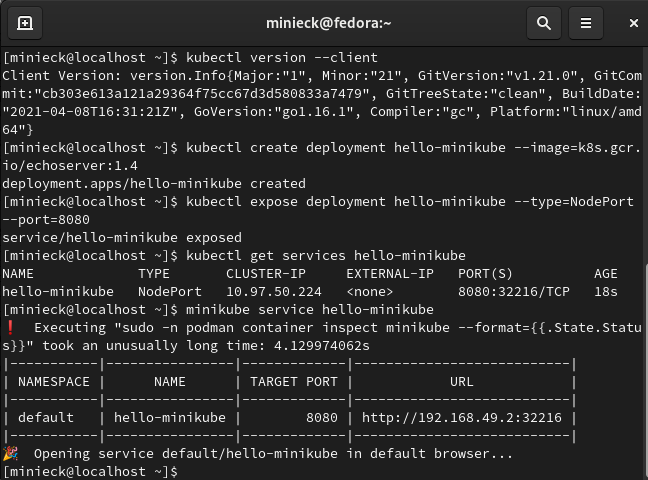
\includegraphics[width=\linewidth]{img/hellokube.png}
    \caption[Het opstarten van een container met kubectl]{Met Kubernetes en kubectl is een container deployment aangemaakt.}
    \label{fig:hellokube}
    \centering
\end{figure}

Om te werken met Kubernetes is er een dashboard weergave die met Minikube opgestart kan worden.
\begin{verbatim}
minikube dashboard
\end{verbatim}
Met deze dashboard kunnen veel van de functionaliteiten van Kubernetes gebruikt worden zonder de CLI te gebruiken. Zo is er via de dashboard een extra pod van de hello-minikube container gestart, wat te zien is in figuur \ref{fig:kubenetesDash}. Iets wat ook interessant is, is dat bij het maken van een container in de dashboard met een formulier kan worden gewerkt. Hierbij is het belangrijk de naam in te stellen en een adres waarvan de image moet worden gepulled. Kubernetes heeft echter geen voor de hand liggende methode om lokaal bewaarde images of private images te gebruiken bij het starten van een container.
\begin{figure}[h]
    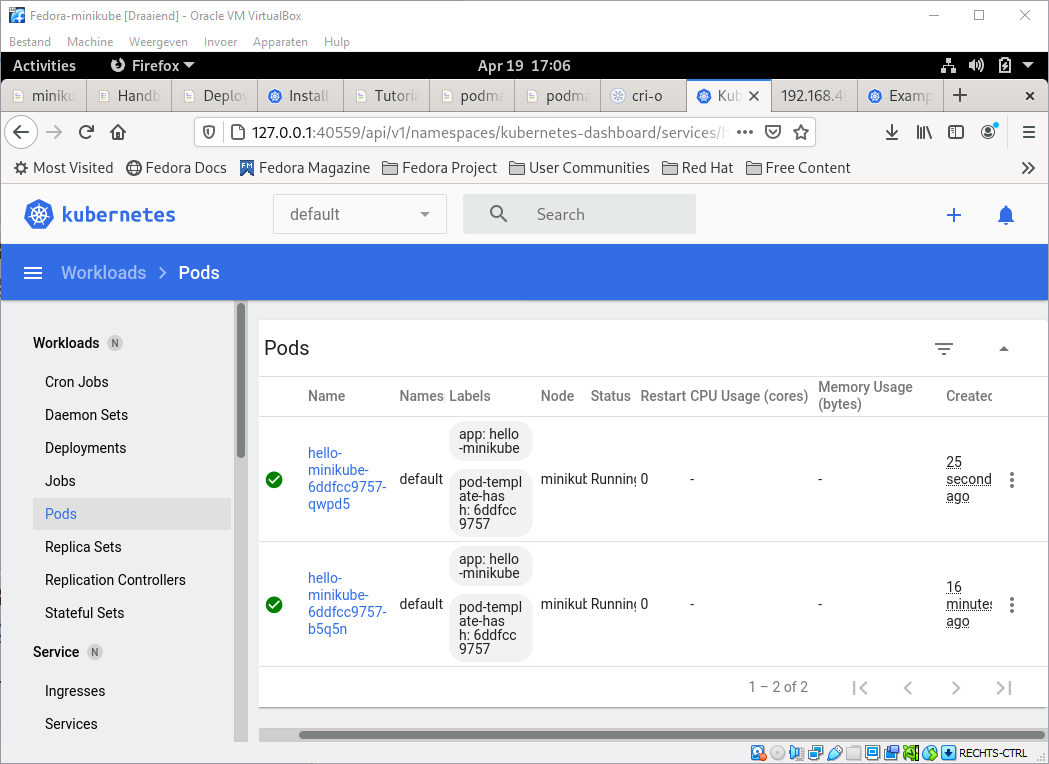
\includegraphics[width=\linewidth]{img/kubenetesDash.png}
    \caption[Het kubernetes Dashboard]{Hier toont de Kubernetes dashboard dat een nieuwe pod van de hellominikube container recent gestart is}
    \label{fig:kubenetesDash}
    \centering
\end{figure}

Vervolgens werd een op basis van een Kubernetes tutorial\footnote{\url{https://kubernetes.io/docs/tutorials/stateful-application/mysql-wordpress-persistent-volume/}} een Wordpress site gemaakt. Dit gebeurt op een gelijkaardige wijze als in Docker Compose met configuratie bestanden die door Kubernetes worden ingelezen. De configuratiebestanden voor de SQL-databank container en de Wordpress container staan in bijlage \ref{K8sql} en \ref{K8wp}. Het primaire bestand dat Kubernetes zal inlezen is een kustomization.yaml. Omdat het wachtwoord gevoelig is zal er gewerkt worden met een secret generator in de kustomization.yaml, dit is te zien in listing \ref{lst:kustomization} . Ook zijn de verwijzingen naar de configuratie van de resources voor de Wordpress site toegevoegd aan dit bestand.
\begin{lstlisting}[caption=inhoud van kustomization.yaml,label=lst:kustomization]
secretGenerator:
- name: mysql-pass
literals:
- password=k8press
resources:
- mysql-deployment.yaml
- wordpress-deployment.yaml
\end{lstlisting}

Eens de kustomization.yml geconfigureerd is kan volgend commando worden uitgevoerd in de map met de 3 bestanden:
\begin{verbatim}
kubectl apply -k ./
\end{verbatim}
Om te controleren of het opstarten gelukt is kan gekeken worden via het dashboard van Kubernetes of met volgende commando’s:
\begin{verbatim}
kubectl get secrets
kubectl get pvc
kubectl get pods
kubectl get services wordpress
\end{verbatim}
Om de Wordpress site te kunnen bezoeken moet deze nog blootgesteld worden naar buiten de cluster. Hiervoor moet Minikube worden gebruikt:
\begin{verbatim}
minikube service wordpress –url
\end{verbatim}
Met de teruggegeven URL kan de Wordpress site in een browser worden bezocht om zo de installatie te beginnen.
Om de site weer te stoppen kan in de folder met de Kustomisation.yml volgend commando worden uitgevoerd om alles te stoppen en verwijderen.
\begin{verbatim}
kubectl delete -k ./
\end{verbatim}

Om te Kubernetes cluster te stoppen moet het volgende commando worden uitgevoerd met Minikube:
\begin{verbatim}
minikube stop
\end{verbatim}

\paragraph{Ervaringen}
Het gebruik van Podman met de GitHub Container Registry was zeer makkelijk en was zoals vermeld volledig gelijkaardig aan de Docker methode. De blogpost gaf een korte uitleg over hoe een container file verder aangepast kan worden om bepaalde zaken te configureren. Jammer genoeg lukte het gebruik van Buildah niet door een conflict tijdens de installatie met de al geïnstalleerde Podman. Buildah zou ook enkel nodig zijn om vanaf nul een nieuwe image te maken, wat inhoudt dat Podman voldoende is als er altijd een bestaande image als vertrekpunt wordt gebruikt.

Het starten van Minikube met Podman vergt wat meer configuratie maar is niet onredelijk. Het gebruikt veel emoticons om zijn berichten te accentueren wat afhankelijk van persoonlijke smaak een minpunt kan zijn. Eens de Minikube Kubernetes gestart is merk je niet meer waarop Kubernetes draait. Ook is Minikube licht genoeg om zonder problemen te werken met 4 GB ram, iets wat de Docker desktop Kubernetes niet kon.

Kubernetes zelf is zeer goed. Er zijn veel gebruiksvoorbeelden voor te vinden en het werkt vlot binnen Minikube. De Dashboard van Kubernetes is ook een zeer groot pluspunt. Het laat een gebruiker toe om de volledige cluster te beheren zonder noodzakelijk via de commandolijn te moeten werken. Ook toont het bij het kiezen van een actie met het dashboard wat het equivalente commando zou zijn om het via command line te doen. Dit is een uitstekende manier om met de CLI commando’s vertrouwd te geraken.


\subsection{Docker engine voor Nomad}
In deze test werd een Ubuntu VM met 4 GB ram en 30 GB harde schijfruimte gebruikt, vooral om te zien of het installeren van Docker zou lukken en omdat deze setup verder al aan alle eisen voor Nomad voldeed.
\paragraph{Installatie en set-up}
De Docker engine installeren en opstarten lukt zonder problemen. Ook het installeren van Nomad zelf gaf geen complicaties.
\paragraph{Ingebruikname}
Na het installeren van de Docker engine werd er eerst getest of alles werkte zoals dit met Docker direct op de laptop lukte, zoals beschreven in sectie \ref{DockerDesktop}. Hierbij werden geen problemen ondervonden.

HashiCorp heeft een korte tutorial\footnote{\url{https://learn.hashicorp.com/collections/nomad/get-started}} die een inleiding geeft tot het werken met Nomad. Eerst moet de lokale agent voor Nomad worden gestart.
\begin{verbatim}
sudo nomad agent -dev -bind 0.0.0.0 -log-level INFO
\end{verbatim}
Eens Nomad gestart is kan in een nieuwe terminal met de agent worden gewerkt. Eerst stelt de tutorial voor om status en member op te halen aan de hand van
\begin{verbatim}
nomad node status
\end{verbatim}
en
\begin{verbatim}
nomad server members
\end{verbatim}

Voor het werken met de jobs die Nomad gebruikt, stel HashiCorp voor om te vertrekken met het volgend commando om in de huidig actieve map een example.nomad te genereren, de inhoud van dit bestand staat in bijlage \ref{nomadjobconfig}. Dit bestand definieert een job om een container van een redis image uit te voeren met de Docker Engine.
\begin{verbatim}
nomad job init
\end{verbatim}
Om deze nieuwe job effectief te starten moet volgend commando worden uitgevoerd, dit is geïllustreerd in figuur \ref{fig:nomadrun}.
\begin{verbatim}
nomad job run example.nomad
\end{verbatim}
De naam die Nomad geeft aan de job eens deze gestart is, is het deel voor de ‘.nomad’ zo kan de status van het voorbeeld worden opgehaald met:
\begin{verbatim}
nomad job status example
\end{verbatim}
Om aan te passen hoeveel instanties van de redis container draaien moet eerst het job bestand worden aangepast. Hiervoor moet op lijn 143 in example.nomad het volgende komen te staan:
\begin{verbatim}
# The "count" parameter specifies the number of the task groups that should
# be running under this group. This value must be non-negative and defaults
# to 1.
+ count = 3
\end{verbatim}
Om de huidig actieve job te doen updaten met de nieuwe vereisten moet de verandering ingepland worden in de scheduler van Nomad.
\begin{verbatim}
nomad job plan example.nomad
\end{verbatim}
Als output van dit commando, te zien in figuur \ref{fig:nomdadplan},wordt de job modify index meegegeven. Om vervolgen de aanpassing door te voeren moet deze worden uitgevoerd aan de hand van:
\begin{verbatim}
nomad job run -check-index 16 example.nomad.
\end{verbatim}
Een andere update wordt ook uitgelegd in de tutorial hiervoor wordt de redis versie in het bestand op Met de dev agent die gestart is wordt een web interface voorzien op http://localhost:4646. Met de web interface kan de huidige status van de Nomad cluster worden geraadpleegd.Echter om iets aan te passen moet gewerkt worden met een job bestand dat in deze interface kan worden geplakt zoals te zien is in figuur \ref{fig:nomdaddash}.

Door de bijkomende barrière van de specifieke HashiCorp configuratie taal is het niet gelukt om een Wordpress site te starten met Nomad.
\begin{figure}[h]
    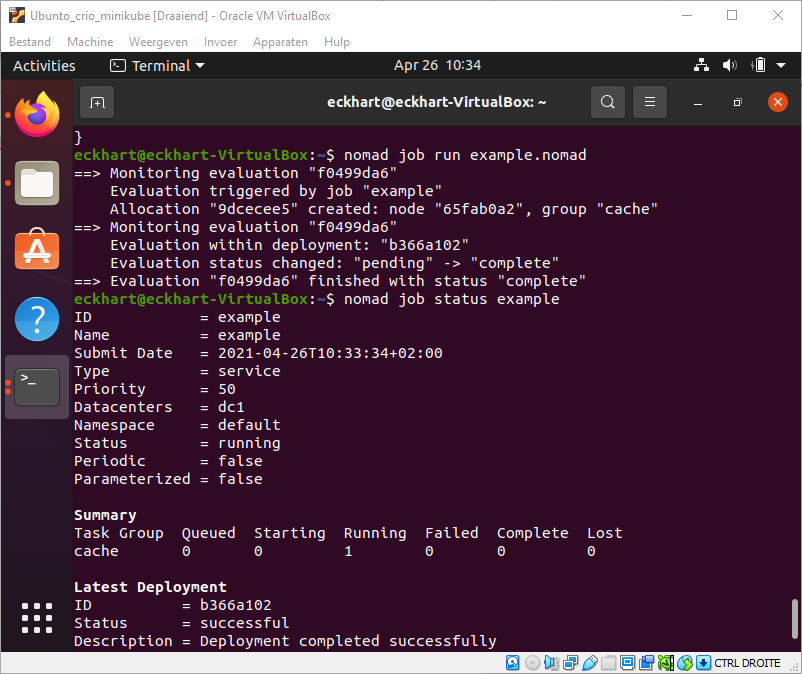
\includegraphics[width=\linewidth]{img/nomadrun.png}
    \caption[Een voorbeeld Nomad job]{Hier wordt via de CLI van Nomad de example.nomad job gestart en de status van opgehaald}
    \label{fig:nomadrun}
    \centering
\end{figure}
\begin{figure}[h]
    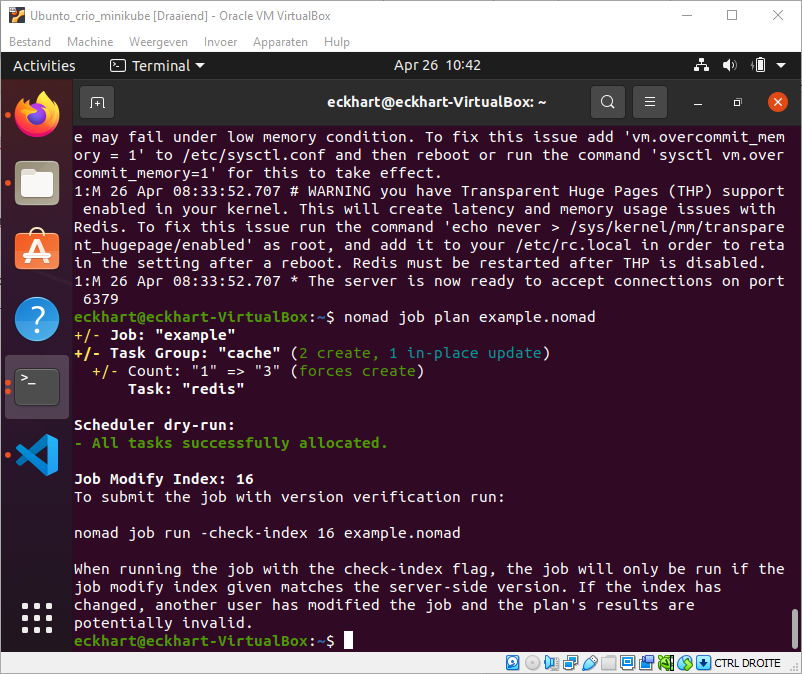
\includegraphics[width=\linewidth]{img/nomadplan.png}
    \caption[Een aangepaste job plannen met Nomad]{Bij het inplannen van een aangepaste job zal Nomad tonen wat aangepast werd en hoe deze uit te voeren.}
    \label{fig:nomdadplan}
    \centering
\end{figure}
\begin{figure}[h]
    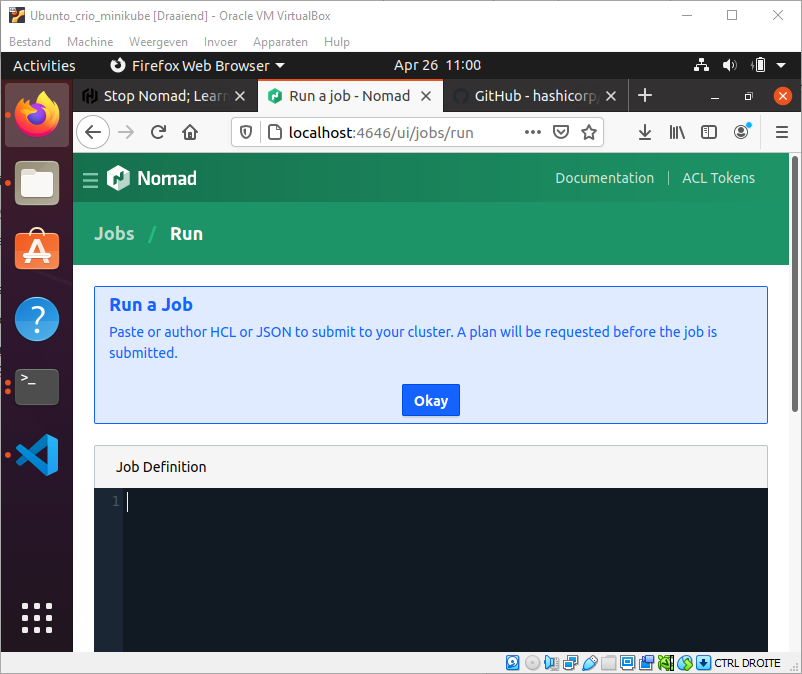
\includegraphics[width=\linewidth]{img/nomdaddash.png}
    \caption[De Nomad dashboard]{De dashboard weergave om een job te starten met Nomad}
    \label{fig:nomdaddash}
    \centering
\end{figure}


\paragraph{Ervaringen}
Door Nomad’s werking met job bestanden voor alle taken is er een duidelijk verschil met Kubernetes. Een groot voordeel is wel dat Nomad meer kan beheren dan enkel containers. Maar het heeft zeker zijn minpunten. Zo is de eigen markup taal voor de configuratie een bijkomende barrière voor het werken met Nomad in vergelijking met de al veelgebruikte YAML die Docker Compose, Podman Compose en Kubernetes allemaal gebruiken. Visual Studio Code heeft wel een extensie voor de HCL configuratie taal die HashiCorp gebruikt, wat het werken met deze .Nomad bestanden vergemakkelijkt. Nomad heeft ook een web browser gebaseerde gebruikersinterface maar deze toont niet wat een equivalent commando voor de command line zou zijn.

\section{Samengevatte resultaten van de softwaretests}
Dit deel vergelijkt samengevattend de verschillende technologieën die getest werden. Enkel voor orchestration is er een duidelijke voorkeur voor Kubernetes als leermiddel.

\subsection{Engines en runtimes}

In basisgebruik lijken Docker en Podman goed op elkaar. De grootste verschillen zitten in de installatie en de eigen werking voor meerdere samenhangende containers. Qua installatie komt Podman standaard geïnstalleerd in Fedora, en moet Docker altijd geïnstalleerd worden. De Docker Compose die afzonderlijk geïnstalleerd moet worden maakt het verbinden van container mogelijk. Het equivalent in Podman met de pods is iets complexer en zelfs met een extra overbrugging van Podman Compose niet voor de hand liggend. Echter deze verbinding tussen containers kan ook volledig gedaan worden in Kubernetes en is bij gebruik van Kubernetes niet meer zo belangrijk.

Verder vormt de Docker Desktop voor het leren maar een kleine meerwaarde. Het is ten eerste niet beschikbaar op Linux systemen. Ten tweede moeten veel cruciale functionaliteiten nog via de command line uitgevoerd worden. Zo geeft de desktop applicatie wel een overzicht van lokale images, maar het maken van een nieuwe image moet via de CLI. Ten derde is de gebundelde Kubernetes zwaarder dan een Kubernetes instantie met Minikube.

\subsection{Repositories}

Tussen de twee gebruikte repositories is er niet meteen één beduidend beter dan de andere. De Docker Hub wordt door zowel Docker als Podman gebruikt als standaard doel om images te pushen. Dit beteken dat er weinig aangepast moet worden om effectief te pushen of te pullen. Echter de Docker Hub zet standaard images publiek en heeft maar één private image mogelijkheid voor gratis accounts. De GitHub Container Registry daarentegen vraagt een beetje extra werk om het doel voor het pushen van een image te selecteren. Het zou wel geen extra account nodig hebben als de student al reeds met GitHub werkt. Over de specifieke kosten en regeling van de GitHub Container Registry kan er echter nog geen definitieve uitspraak gedaan worden omdat deze nog in bèta fase is. Indien echter dezelfde limiet van 500 mb voor private containers zou gelden als bij de rest van de GitHub packages dan zou deze te klein zijn om meer te kunnen bevatten dan één of enkele private images.

\subsection{Orchestration}

Voor orchestration is Kubernetes de beste van de twee geteste orchestration softwares voor het werken met containers. Zo heeft het een dashboard weergave die niet alleen de noodzaak om te werken via de command line minimaliseert, het toont ook bij het uitvoeren van taken via deze dasboard de equivalente commando’s om het via de CLI te doen. Om met Kubernetes te leren werken is Minikube ook een pluspunt. Minikube helpt om een lokale Kubernetes cluster op te starten en beheren. Verder kan Minikube ook de juiste verbindingen maken om een keuze aan achterliggende runtimes te hebben. Minikube heeft de beste ondersteuning voor Docker als engine maar kan met wat extra configuratie en het installeren van Cri-o als hulpstuk ook met Podman als driver werken. Een groot minpunt is dat Kubernetes moeilijk toelaat om containers te draaien op basis van lokaal bewaarde images of privé bewaard in een repository.

Om specifiek met containers te werken is Nomad minder aan te raden. De specifieke HashiCorp configuratie taal is mogelijks een belangrijke barrière in het leerproces. Het kan dat een student de YAML configuratie taal die Kubernetes gebruikt nog niet gezien heeft, maar de kans is groter dat de student ook YAML elders zal tegenkomen dan de HashiCorp markup. Wat ook het leren nadelig zou beïnvloeden vergeleken met Kubernetes is dat de Nomad dashboard niet de equivalente CLI commando’s toont. Dit is deels te verklaren door de aanpak van Nomad om aanpassingen aan je draaiende containers te doen op basis van jobs, die telkens geschreven moeten worden in de HashiCorp configuratie taal.
